%pdflatex -halt-on-error -aux-directory=tmp -output-directory=tmp rapport.tex%

\documentclass{article}
\usepackage{amsmath}
\usepackage[utf8]{inputenc}
\usepackage[T1]{fontenc}
\usepackage{graphicx}
\usepackage{hyperref}
\usepackage[francais]{babel}
\usepackage{listings}
\usepackage{xcolor}

\definecolor{codegreen}{rgb}{0,0.6,0}
\definecolor{codegray}{rgb}{0.5,0.5,0.5}
\definecolor{codepurple}{rgb}{0.58,0,0.82}
\definecolor{backcolour}{rgb}{0.95,0.95,0.92}

\lstdefinestyle{mystyle}{
    language=python,
    backgroundcolor=\color{backcolour},   
    commentstyle=\color{codegreen},
    keywordstyle=\color{magenta},
    numberstyle=\tiny\color{codegray},
    stringstyle=\color{codepurple},
    basicstyle=\ttfamily\footnotesize,
    breakatwhitespace=false,         
    breaklines=true,                 
    captionpos=b,                    
    keepspaces=true,                 
    numbers=left,                    
    numbersep=5pt,                  
    showspaces=false,                
    showstringspaces=false,
    showtabs=false,                  
    tabsize=2
}

\lstset{style=mystyle}

\title{Théorie des langages II - TD1}
\author{Wassim SAIDANE}
\date{}

\begin{document}
    \pagenumbering{gobble}
    \maketitle
    \pagenumbering{arabic}
    \section*{Question 1}
    Montrer  que  le  langage $a^nb^n(\text{pour } n \ge 1)$  n’est  pas  rationnel.  Concevoir  un automate à pile qui reconnît ce langage. \\
    \\
    Langage rationnel \footnote{D'après wikepedia} : \\
    \begin{itemize}
        \item Ce sont les langages décrits par les expressions régulières ou rationnelles, d'où le nom de langages réguliers.
        \item Ce sont les langages obtenus, à partir des lettres et de l'ensemble vide, par les opérations rationnelles, à savoir l'union, le produit et \href{https://fr.wikipedia.org/wiki/Étoile_de_Kleene}{l'étoile de Kleene}, d'où le nom de langages rationnels.
        \item ce sont les langages reconnus par des automates finis, d'où le nom de langages reconnaissables.
    \end{itemize} 
    Soit le langage $L=\{a^nb^n \mid n \ge 0\}$ sur l'alphabet $A=\{A,B\}$. Supposons \underline{par l'absurde} que $L$ est rationnel. \\
    \href{https://fr.wikipedia.org/wiki/Lemme_de_l%27étoile}{\underline{Par le lemme d'itération}}, $\{\exists x,y,z \mid $w=xyz$\}$, $\mid xy \mid \le p, \mid y \mid \ge 1$ 
    et $\forall i \ge 0, xy'z \in L$. \\
    Comme $\mid xy \mid \supseteq p$, alors $w=a^la^{l'}a^{l''}b^p$ où $x=a^l$, $y=a^{l'}$, $z=a^lb^p$ $l' \ge 1$. Si on applique la proposition 4 ($\forall i \ge 0, xy^iz \in L$ )
    du lemme d'itération avec $i=0$ on obtient $a^la^{l''}b^p \in L,$ or $l+l'' < P$. ($l+l'+l''=p, l' \ge 1$) \\
    CONTRADICTION. \\
    $L$ n'est donc pas un langage rationnel. \\
    \\
    \url{https://fr.wikipedia.org/wiki/Automate_à_pile#Un_exemple}

    Pour définir l'automate à pile, nous allons définir des règles de transition (q, y, z, p, h) où :
    \begin{itemize}
        \item q est l'état de départ
        \item y est la lettre utilisée
        \item z est le symbole qu'on dépile
        \item p est l'état d'arrivé
        \item h est le symbole qu'on empile
    \end{itemize}

    Par exemple, soit les 4 règles suivantes :
    \begin{enumerate}
        \item (q, a, $\omega$, q, A)
        \item (q, a, A, q, AA)
        \item (q, $\epsilon$, A, p, A)
        \item (p, n, A, p, $\epsilon$)
    \end{enumerate}
    
    La première règle nous dit qu'en prenant 'a' à partir de l'état 'q', on reste en 'q' en n'ayant rien dépilé
    mais en ayant empilé 'A'.
    Il n'y a pas d'état final, la reconnaissance du mot se fait par pile vide (sauf le mot vide car $n\geq0$)

    Voici la représentation de l'automate à pile (MERCI WIKIPEDIA) :\\
    
    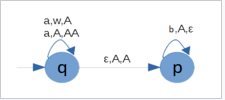
\includegraphics[width=\textwidth]{images/question1_automate.PNG}

\end{document}
